\section{Förderband}
\label{sec:Foerderband}
	Da die Beschleunigungsräder durch den Abwurf abgebremst werden, müssen sie nach 
	jedem Wurf wieder auf Nenndrehzahl gebracht werden. Um dafür genügend Zeit zu 
	haben, erfolgt die Zuführung der Bälle in zeitlichen Abständen. Ein weiteres 
	Kriterium für eine konstante Wurfweite, ist eine gleichbleibende Geschwindigkeit 
	mit der die Bälle zwischen die Beschleunigungsräder kommen. Der Antrieb des 
	Förderbandes erfolgt mit einem DC-Motor, siehe Kapitel 7.1. Die Drehzahl ist 
	mittels einer Zahnradpaarung mit i=5 übersetzt, um das benötigte Drehmoment an 
	die Antriebswelle des Förderbandes zu übertragen. Die Antriebswelle und die Achse 
	sind einteilig aus Aluminium gedreht. Welle und Achse sind mittels Kugellager 
	in den Seitenplatten gelagert. Die Auflagefläche des Riemens auf der Antriebswelle 
	ist bombiert gefertigt. Dadurch wird ein seitliches Abrutschen des Riemens im 
	Betrieb verhindert. Auf dem Förderband, welches ein Flachbandriemen ist, sind 
	Führungsschaufeln angebracht. Durch den Abstand dieser Schaufeln, ergeben sich 
	die kurzen Pausen um die Motoren wieder hochzudrehen. Die Führungsschaufeln sind 
	so ausgerundet, dass der Ball möglichst lange geführt werden kann ohne die 
	Beschleunigungsräder zu berühren. Die Schaufeln sind aus 1 mm Aluminium Blech 
	gefertigt und wurden im ersten Stadium auf dem Riemen aufgeklebt.-……??- Aus 
	diversen Testversuchen der Ballzuführung wurde erkannt, dass für einen idealen 
	Abwurf die Tennisbälle mit beiden Beschleunigungsräder gleichzeitig in Kontakt 
	kommen müssen. Somit ist es notwendig die Bälle zunächst unter dem oberen 
	Beschleunigungsrad hindurch und anschliessend in einem 45° Winkel nach oben 
	zuzuführen. Dazu dient ein Führungselement, welches auf beiden Seiten des 
	Acrylglases angebracht ist. Diese Führungselemente sind an die Form der Tennisbälle 
	angepasst und mittels 3D Druck hergestellt worden. 

	\begin{figure}[h!]
    	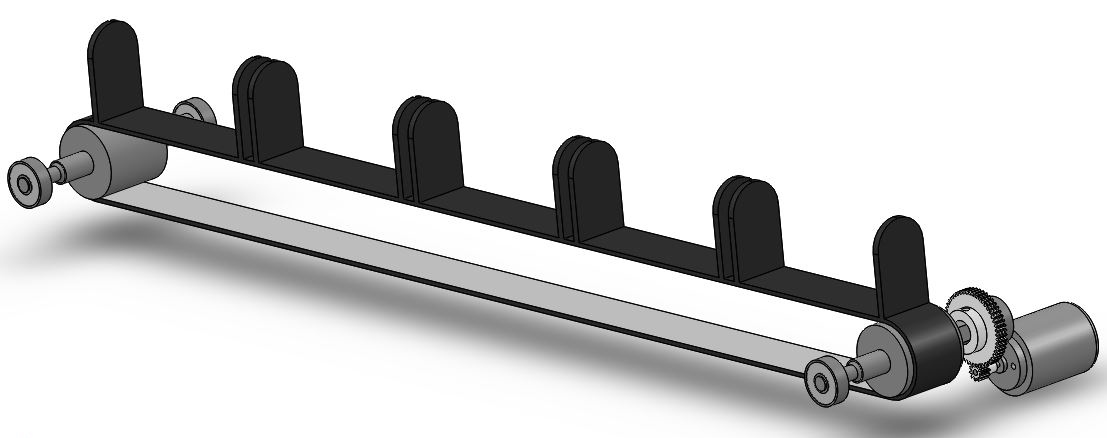
\includegraphics[width=0.9\textwidth,clip,trim=0mm 0mm 0mm 0mm]
    	{Enddokumentation/Bilder/Foerderband.jpg}
    	\centering
    	\caption{Aufbau des Förderbandes}
    	\label{abb:Foerderband}
 \end{figure}

\subsection{Ansteuerung DC-Motor}
\label{sec:FoerderbandAnsteuerung}
    Die Ansteuerung des Motors, der das Förderband antreibt, erfolgt mittels PWM. Auf diese 
    Weise lässt sich die Drehzahl und somit die Nachführgeschwindigkeit einstellen. Das 
    Band muss nur in eine Richtung angetrieben werden, wodurch die Ansteuerung einfacher 
    realisiert werden kann. Das Schema ist in Abbildung \ref{abb:SchemaAnsteuerung} 
    ersichtlich. Im wesentlichen besteht diese Ansteuerung aus einem Vortreiber und einem 
    Schalter. Der Treiber bewirkt ein möglichst schnelles und effizientes Öffnen und Schliessen des Schalters. Auf diese Weise reduziert man die Schaltverluste. 
    \begin{figure}[h!]
    	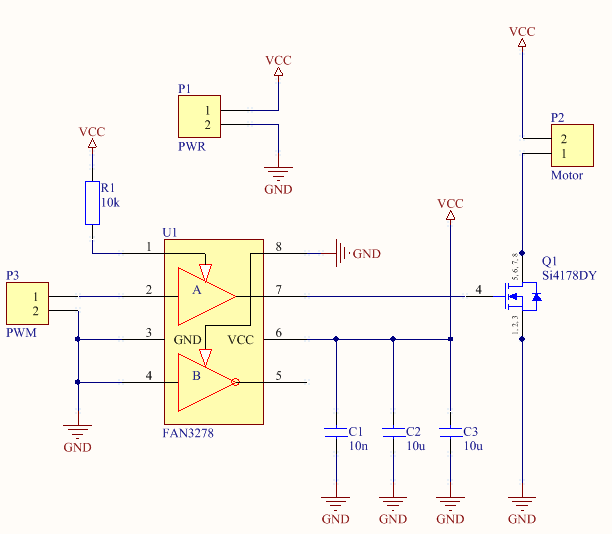
\includegraphics[width=0.7\textwidth,clip,trim=0mm 2mm 0mm 7mm]
    	{Enddokumentation/Bilder/Schema_DC-Ansteuerung.png}
    	\centering
    	\caption{Schema des Förderbandansteuerung}
    	\label{abb:SchemaAnsteuerung}
    \end{figure}
    
\newpage